\section{Referencial Teórico}\label{sec:referencial}

Para avaliar a qualidade, a capacidade ou a ``inteligência'' de determinado modelo de IA, são realizados repetidos testes sistemáticos. Quanto maior a cobertura dos testes, mais as métricas são precisas para avaliar a qualidade da tarefa realizada pelo modelo, seja ela classificação, regressão ou geração de conteúdo. Entretanto, sobretudo em modelos generativos, é inviável exaurir todo o espaço de entradas restando a incerteza sobre quando e onde erros podem acontecer \citep{Yu2025}. Sendo assim, a principal pergunta que resta é: ``podemos confiar no modelo?''. Ou talvez, de modo mais preciso: ``quais certezas precisamos ter para confiar no modelo?''.

O ato de confiar em algo ou em alguém exige certo grau de vulnerabilidade. Nesse sentido, disponibilizar informações relevantes e verificáveis, que permitam julgar o quanto essa vulnerabilidade é razoável, é essencial para que haja confiança. Esse processo é denominado transparência. Entretanto, paradoxalmente, a transparência total pode minar a confiança, pois elimina a vulnerabilidade que a sustenta (se tudo pode ser auditado e verificado sem risco, não há confiança, mas apenas verificação). No que diz respeito à IA é importante ressaltar que a confiança depositada nela ainda não apresenta valor relacional, mas sim instrumental, visto que contamos com ela para nos servir como ferramenta e não como parte de uma relação social \citep{Mitchell2025}.

Quando aceitamos os resultados de um modelo de IA sem ter acesso a nenhuma informação sobre como ele chega às suas conclusões, estamos diante de uma situação análoga à de confiar em um especialista humano que, por experiência e prática, desenvolveu uma intuição confiável. Assim, a confiança se apoia na expectativa de competência construída a partir de treinamento prévio e acúmulo de experiência, não na transparência do processo interno, o que pode ser considerado ingênuo visto que não podemos avaliar ou mensurar todos os casos de teste para alguns modelos. Por consequência, para podermos confiar em determinado modelo de IA é preciso que ele seja transparente, é preciso conseguir obter, de forma clara e compreensível, as informações sobre como ele toma suas decisões, permitindo que usuários verifiquem e avaliem sua confiabilidade \citep{Mitchell2025}.

\subsection{Explicabilidade, interpretabilidade e compreensibilidade}

Inteligência artificial explicável (XAI) refere-se ao desafio de reduzir a opacidade dos modelos \textit{black-box}, atribuindo-lhes certo grau de transparência \citep{Longo2024, ICO2022}. Para isso, diversas técnicas de geração de explicações foram propostas nos últimos anos, buscando tornar mais compreensíveis os critérios e processos que orientam as previsões e decisões desses sistemas \citep{Mersha2024, Guidotti2022, Longo2024, Marino2025}. Existe uma distinção importante entre essas técnicas no que diz respeito ao momento e à forma como a explicação é produzida. Em alguns casos, a explicação é incorporada ao próprio processo de construção do modelo, durante o treinamento. Em outros casos, o modelo já está totalmente treinado e as explicações são geradas de maneira posterior. Dessa forma, as técnicas de geração de explicações podem ser classificadas em:

\begin{itemize}
    \item \textbf{\textit{Ante-hoc:}} métodos que geram uma explicação durante a fase de treinamento e desenvolvimento ou durante a fase de uso \citep{Marino2025}.
    \item \textbf{\textit{Post-hoc:}} métodos que geram uma explicação com base na entrada e saída de um modelo \textit{black-box} já treinado. Esses métodos podem contar com outros modelos de inteligência artificial \citep{Guidotti2022}.
\end{itemize}

A escolha entre técnicas \textit{ante-hoc} e \textit{post-hoc} depende do modelo para o qual se busca a explicação. Em muitos casos, é possível empregar ambas de forma complementar, ampliando a qualidade, a abrangência e a profundidade das informações oferecidas sobre o processo de tomada de decisão \citep{Mersha2024}. A técnica também pode ser localizada para explicar um conjunto de amostras preditas (explicação local), ou pode ser generalizada para tentar explicar o comportamento global do modelo (explicação global). Métodos \textit{post-hoc} também podem ser diferenciados de acordo com sua aplicabilidade. Aqueles restritos a apenas um tipo específico de estrutura ou modelo são denominados modelo-específicos, enquanto aqueles que podem ser empregados independentemente da estrutura do modelo são denominados modelo-agnósticos \citep{Longo2024}.

Os termos explicabilidade e interpretabilidade são muito relacionados ao conceito de transparência, entretanto não apresentam uma definição clara na literatura de XAI. Esses termos acabaram sendo definidos de maneiras distintas por diferentes autores, sendo que alguns trabalhos acabam utilizando-os de forma intercambiável \citep{Mersha2024}. Além disso, o uso desses conceitos em diferentes áreas acaba gerando mais ruído em suas definições. A ausência de consenso gera ambiguidade e confusão, tanto em relação aos próprios conceitos quanto com relação a outros termos que deles dependem \citep{Erasmus2021}. Veja que os próprios termos \textit{ante-hoc} e \textit{post-hoc}, definidos previamente, dependem da definição daquilo que se entende como explicabilidade.

O trabalho de \cite{Erasmus2021} apresenta uma distinção entre os termos interpretabilidade, explicabilidade e compreensibilidade a partir da estrutura geral das explicações científicas, na qual o \textit{explanandum} (o fenômeno a ser explicado) é relacionado ao \textit{explanans} (os fatos e argumentos que o sustentam). Assim, explicabilidade refere-se à possibilidade de estabelecer uma relação entre fenômeno e fundamentos teóricos ou empíricos que o sustentem, independentemente da complexidade do sistema. A interpretabilidade, por sua vez, corresponde ao processo de tornar uma explicação já existente mais clara, estruturada e adaptada ao público-alvo ou ao contexto em que será utilizada. Por fim, a compreensibilidade está ligada à capacidade do indivíduo de efetivamente entender o fenômeno a partir da explicação recebida. Nesse caso, a complexidade do sistema exerce influência direta: mesmo que se mantenha o mesmo explicador, o aumento da complexidade pode reduzir o nível de entendimento do público, comprometendo a compreensibilidade.

Essas distinções têm consequências práticas. Quando uma decisão apoiada por sistemas de IA nos prejudica, surge a questão de como atribuir responsabilidade. Apenas manter um humano no processo decisório não é suficiente, pois, sem acesso às razões que fundamentam a recomendação do sistema, essa pessoa não possui as condições epistêmicas necessárias para ser considerada moralmente responsável. Nesse sentido, explicações tornam-se indispensáveis, pois devem oferecer transparência sobre o funcionamento interno da IA e permitir que os usuários compreendam e avaliem criticamente as decisões apresentadas. Esse tipo de explicação possibilita que os humanos no circuito possam deliberar, concordar ou discordar e, assim, assumir responsabilidade moral pelas decisões. Portanto, a interpretabilidade em IA não se restringe a uma ferramenta para aumentar a confiança instrumental, mas constitui uma exigência fundamental para prevenir lacunas de responsabilidade \citep{Baum2022}.

Entre as dimensões que devem ser consideradas para que uma explicação seja adequada, talvez a mais fundamental seja a causalidade, que constitui um traço central do pensamento humano \citep{Bender2020} e cujo modelo intervencionista é muito utilizado em explicações de XAI atualmente \citep{Guidotti2022}. De acordo com \cite{Pearl2009}, é possível evidenciar efeitos causais entre variáveis por meio de uma intervenção, representada pela operação \(do(\cdot)\). Dadas duas variáveis \(A\) e \(B\), em vez de observar a probabilidade condicional \(P(B \mid A)\), intervém-se em \(A\) para fixá-la em determinado valor, obtendo \(P(B \mid do(A))\), o que remove a influência de variáveis confundidoras e revela possíveis efeitos causais. Por esse motivo, recomenda-se que sistemas de IA interpretáveis explicitem as relações de causa e efeito presentes em suas decisões, tanto para assegurar a transparência causal quanto para possibilitar a adequada atribuição de responsabilidade \citep{Bender2020, Baum2022}. Além disso, métodos de XAI deveriam declarar explicitamente qual tipo de explicação produzem, visto que usuários só compreendem o que lhes é apresentado quando reconhecem a estrutura explicativa subjacente, e o campo ainda carece de clareza conceitual nesse aspecto \citep{Graff2025, Mersha2024, Pawlicki2024}.

Uma das formas mais diretas de expressar uma explicação causal é por meio de contrafactuais, que respondem à pergunta ``o que teria acontecido se a entrada fosse diferente?'' \citep{Pearl2009, Wachter2018}. Considerando um modelo \(f\) e uma instância \(x\) tal que \(y = f(x)\), um contrafactual \(x'\) é uma instância tal que \(y' = f(x')\) e \(y \neq y'\). Além disso, a distância entre \(x\) e \(x'\) deve ser mínima, de modo que a diferença entre as duas instâncias indique o que precisaria mudar para que a decisão mudasse \citep{Guidotti2022}. Explicações desse tipo são contrastivas, isto é, explicam por que o modelo decidiu \(y\) em vez de \(y'\), o que corresponde à forma como humanos costumam pedir e oferecer explicações \citep{Miller2019}. Uma estratégia comum é tomar como contrafactual a instância mais próxima de \(x\), entre as já observadas, que recebe uma decisão diferente \citep{KeaneSmyth2020, Brughmans2024}, o que depende inteiramente da noção de distância adotada. Veja que essa definição utiliza apenas as entradas e as saídas de \(f\), sendo portanto modelo-agnóstica.

\subsection{Interpretabilidade mecanicista e métodos geométricos}

Métodos de XAI buscam desenvolver algoritmos capazes de gerar explicações para sistemas de decisão baseados em IA. À medida que esses sistemas se tornam mais complexos, técnicas de interpretabilidade mecanicista tendem a se mostrar mais úteis. Essas técnicas partem da premissa de que sistemas de IA suficientemente complexos são mais bem compreendidos a partir de perspectivas semelhantes às utilizadas no estudo de sistemas biológicos. Isso exige a aplicação de estratégias familiares às ciências biológicas, como reconhecimento de padrões, decomposição funcional, localização e manipulação experimental sistemática \citep{Kastner2024}.

No contexto dos sistemas de IA, as técnicas de reconhecimento de padrões consistem em um conjunto de atividades epistêmicas orientadas por normas compartilhadas. Entre essas atividades, destacam-se: (1) a decomposição, que consiste em fragmentar um fenômeno em seus elementos constitutivos, geralmente de modo recursivo, a fim de identificar características funcionais em diferentes níveis, (2) a localização, entendida como a atribuição de uma funcionalidade a uma parte específica do sistema supostamente responsável por sua implementação, e (3) a recomposição, que envolve reconstruir o sistema de maneira funcionalmente informada \citep{Kastner2024}.

Essas estratégias têm sido exploradas em trabalhos recentes de empresas como \textit{Anthropic} e \textit{OpenAI}. \cite{Ameisen2025} propuseram o \textit{circuit tracing}, que substitui partes do modelo original por componentes mais interpretáveis e constrói grafos de atribuição entre \textit{features} esparsamente ativas, permitindo rastrear as cadeias de raciocínio do modelo para entradas específicas. De forma complementar, \cite{DupreLaTour2025} utilizaram atribuição diferencial sobre \textit{features} latentes de \textit{sparse autoencoders} para identificar as \textit{features} causalmente responsáveis por comportamentos desalinhados. Veja que ambos os métodos dependem de um modelo substituto ou de um dicionário de \textit{features} treinado à parte, enquanto o método proposto neste trabalho opera diretamente sobre quantidades produzidas pelo próprio modelo.

\begin{figure}[hbt!]
    \centering
    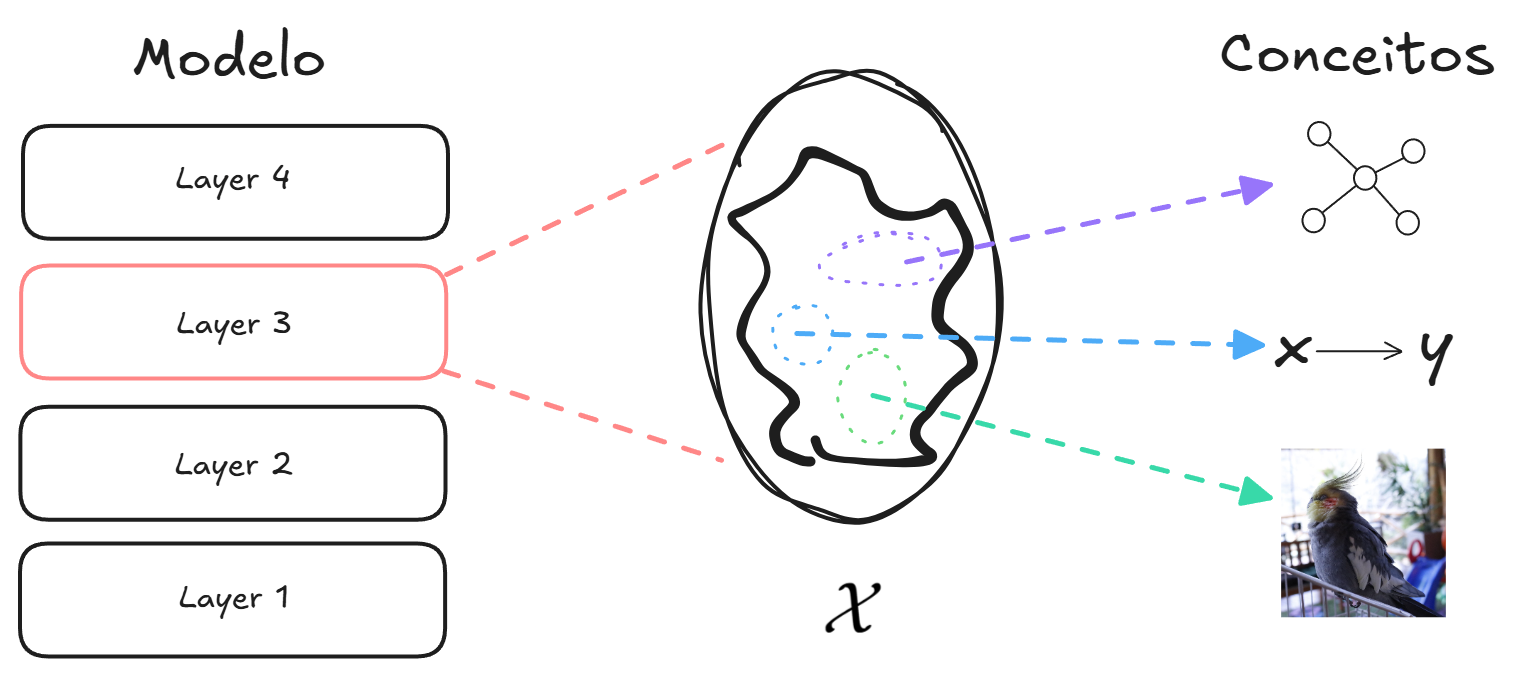
\includegraphics[width=\textwidth]{img/Concepts.png}
    \caption{Representação esquemática da extração de conceitos a partir de uma camada intermediária do modelo: a Layer 3 é projetada em um espaço latente, no qual diferentes regiões correspondem a conceitos distintos, associados tanto a estruturas abstratas quanto a padrões funcionais e semânticos.}
    \label{fig:concepts}
\end{figure}

Métodos geométricos de interpretabilidade, por sua vez, fundamentam-se na estrutura matemática dos espaços de representação internos dos modelos, utilizando ferramentas de geometria, teoria espectral e análise funcional para caracterizar o comportamento da rede. O \textit{geometric deep learning} fornece a base teórica dessa abordagem ao formalizar a aprendizagem profunda sobre domínios não euclidianos, como grafos e variedades \citep{Cao2020, Bronstein2017}. Nesse sentido, um modelo pode ser tratado como o próprio objeto geométrico a ser analisado, de modo que a geometria dos espaços de funções resultantes é utilizada para diagnosticar e explicar as decisões do modelo. A Figura \ref{fig:concepts} ilustra essa ideia de forma esquemática, em que a representação de uma camada intermediária é projetada em um espaço no qual regiões distintas correspondem a conceitos distintos.

\subsection{Um método de interpretabilidade baseado em \textit{kernels}}\label{subsec:metodo_proposto}

Este trabalho propõe um método geométrico de interpretabilidade baseado em \textit{kernels}. De acordo com a tipologia apresentada anteriormente, trata-se de um método \textit{post-hoc}, pois opera sobre um modelo já treinado sem interferir no seu treinamento, e modelo-agnóstico, pois a sua formulação exige apenas que cada amostra possa ser descrita por um conjunto de fontes de informação sobre as quais se define um \textit{kernel}, sem supor nenhuma arquitetura. A escolha das fontes, por sua vez, constitui uma instanciação do método, que pode utilizar estados internos de uma rede neural ou o caminho percorrido em uma árvore de decisão. O método produz explicações locais, sobre amostras e pares de amostras, e globais, sobre a organização do espaço de representação. Além disso, a distância que ele induz define quais instâncias são próximas, o que permite escolher contrafactuais e atribuir a diferença entre uma amostra e o seu contrafactual às variáveis de entrada. O método é descrito ao longo das próximas seções: o tensor de similaridade que o fundamenta é desenvolvido na Seção \ref{sec:tensor_rkhs}, o procedimento de construção da matriz de Gram é apresentado na Seção \ref{sec:kernel_pipeline} e a energia espectral utilizada em suas leituras é definida na Subseção \ref{subsec:spectral}.

Por fim, o método se diferencia das técnicas de análise representacional que também operam sobre matrizes de similaridade, como a análise de similaridade representacional (RSA) \citep{Kriegeskorte2008} e o alinhamento centrado de \textit{kernels} (CKA) \citep{Kornblith2019}. Essas técnicas são utilizadas para comparar representações, sejam elas de duas camadas, de dois modelos ou de um modelo e um sistema biológico, e resumem essa comparação em um único valor de semelhança. O método proposto, por sua vez, não tem como objetivo comparar representações, mas sim construir um espaço de representação a partir de fontes heterogêneas de um mesmo modelo e, a partir desse espaço, gerar afirmações sobre o comportamento do modelo que o originou. A relação formal entre o método e a CKA é examinada nos resultados.

\section{Núcleo Reprodutor em Espaços de Hilbert}\label{sec:rkhs}

O método proposto neste trabalho é construído sobre a teoria de \textit{kernels} formalizada por \cite{Aronszajn1950}, que faz parte da teoria clássica de aprendizagem de máquina. Os Espaços de Hilbert com Núcleo Reprodutor (\textit{Reproducing Kernel Hilbert Spaces} ou RKHS) fornecem a base funcional que conecta a noção de similaridade entre dados, expressa por \textit{kernels}, à geometria dos espaços de representação internos dos modelos. Ao garantir que a avaliação pontual de funções seja uma operação contínua, os RKHS permitem que propriedades geométricas do espaço de funções sejam exploradas de forma estável, o que é essencial para a construção de métodos de interpretabilidade que operem diretamente sobre as representações aprendidas. As definições apresentadas a seguir seguem \cite{Aronszajn1950} e \cite{Scholkopf2001}.

\textbf{Espaço de Hilbert:} Um espaço de Hilbert $\mathcal{H}$ é um espaço vetorial munido de um produto interno $\langle \cdot, \cdot \rangle_{\mathcal{H}}: \mathcal{H} \times \mathcal{H} \to \mathbb{R}$ que é completo em relação à norma induzida $\|f\|_{\mathcal{H}} = \sqrt{\langle f, f \rangle_{\mathcal{H}}}$. A completude significa que toda sequência de Cauchy, isto é, toda sequência cujos termos ficam arbitrariamente próximos entre si, converge para um elemento do próprio espaço, de modo que $\mathcal{H}$ não possui ``lacunas''.

\textbf{Núcleo Reprodutor:} Um núcleo reprodutor (\textit{kernel}) é uma função $k: \mathcal{X} \times \mathcal{X} \to \mathbb{R}$ simétrica, isto é, $k(x, x') = k(x', x)$ para todo $x, x' \in \mathcal{X}$, e positivamente definida, o que significa que, para qualquer conjunto finito de pontos $\{x_1, x_2, \dots, x_n\} \subset \mathcal{X}$ e quaisquer escalares $c_1, c_2, \dots, c_n \in \mathbb{R}$,

\begin{equation}\label{eq:pos_def}
    \sum_{i=1}^{n} \sum_{j=1}^{n} c_i \, c_j \, k(x_i, x_j) \geq 0.
\end{equation}

A exigência de definição positiva decorre diretamente da interpretação do \textit{kernel} como um produto interno em algum espaço de características. Considere um mapeamento $\phi: \mathcal{X} \to V$ tal que $k(x_i, x_j) = \langle \phi(x_i), \phi(x_j) \rangle_V$. A norma ao quadrado de um vetor $v = \sum_i c_i \, \phi(x_i) \in V$ é dada por

\begin{equation}\label{eq:kernel_norm}
    \|v\|^2 = \left\langle \sum_i c_i \, \phi(x_i),\; \sum_j c_j \, \phi(x_j) \right\rangle_V = \sum_{i=1}^{n} \sum_{j=1}^{n} c_i \, c_j \, k(x_i, x_j),
\end{equation}

\noindent de modo que a condição \eqref{eq:pos_def} equivale à não-negatividade da norma, propriedade necessária de qualquer produto interno. Na prática, calcular $\phi$ explicitamente pode ser inviável ou computacionalmente custoso. O \textit{kernel} contorna esse problema ao computar o produto interno no espaço transformado diretamente a partir dos pontos originais, sem jamais construir $\phi$ de forma explícita. Esse procedimento é conhecido como \textit{kernel trick} \citep{Scholkopf2001} e está ilustrado na Figura \ref{fig:kernel_trick}.

\begin{figure}[!htbp]
  \centering
  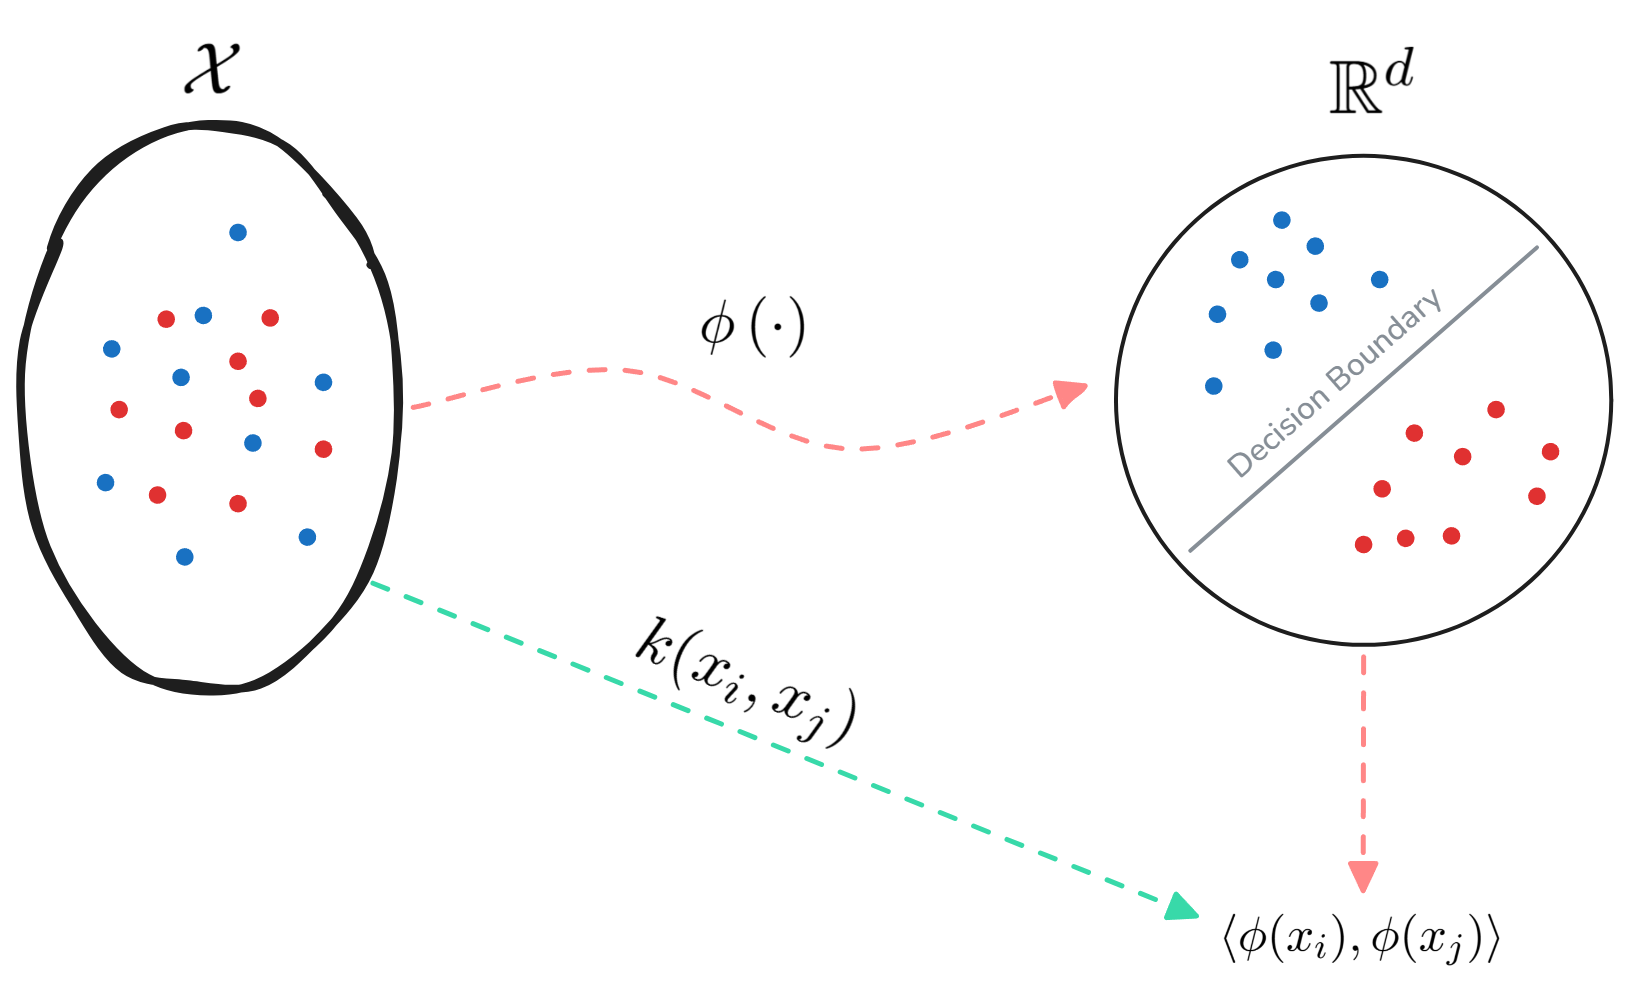
\includegraphics[width=\textwidth]{img/Kernel.png}
  \caption{O mapa de características $\phi$ leva os dados do espaço de entrada $\mathcal{X}$ para um espaço de dimensão maior $\mathbb{R}^d$\, onde as classes se tornam linearmente separáveis. Na prática, calcular $\phi$ explicitamente pode ser inviável ou computacionalmente custoso. O \textit{kernel} $k(x_i, x_j) = \langle \phi(x_i), \phi(x_j) \rangle$ contorna esse problema: ele computa o produto interno no espaço transformado diretamente a partir dos pontos originais, sem nunca construir $\phi$ (esse é o chamado ``\textit{kernel trick}'')}
  \label{fig:kernel_trick}
\end{figure}

\textbf{Matriz de Gram:}\label{def:gram} Dados $n$ pontos $\{x_1, x_2, \dots, x_n\} \subset \mathcal{X}$ e um \textit{kernel} $k$, a matriz de Gram é a matriz $K \in \mathbb{R}^{n \times n}$ cujas entradas são $K_{ij} = k(x_i, x_j)$. Pelo \textit{kernel trick}, cada entrada corresponde ao produto interno $\langle \phi(x_i), \phi(x_j) \rangle_V$ no espaço de características, de modo que $K$ codifica todas as relações de similaridade entre os pontos sem que $\phi(\cdot)$ precise ser obtido. A condição de definição positiva do \textit{kernel} garante que $K$ é semidefinida positiva, isto é, $c^\top K c \geq 0$ para todo $c \in \mathbb{R}^n$, que é a mesma condição imposta pelo produto interno expressa em formato matricial.

\textbf{Kernel Produto:} Dado um conjunto $\{k_1, k_2, \dots, k_n\}$ de \textit{kernels} positivamente definidos, com cada $k_i: \mathcal{X}_i \times \mathcal{X}_i \to \mathbb{R}$, o \textit{kernel} produto definido sobre $\mathcal{X} = \mathcal{X}_1 \times \mathcal{X}_2 \times \cdots \times \mathcal{X}_n$ é dado por

\begin{equation}\label{eq:kernel_prod}
    k(x, x') = \prod_{i=1}^{n} k_i(x_i, x_i'),
\end{equation}

\noindent onde $x = (x_1, \dots, x_n)$ e $x' = (x_1', \dots, x_n')$. Veja que, em termos matriciais, a matriz de Gram de $k$ é o produto de Hadamard $K_1 \circ K_2 \circ \cdots \circ K_n$ das matrizes de Gram dos fatores. Como o produto de Hadamard de matrizes semidefinidas positivas é semidefinido positivo, pelo teorema de Schur \citep{Schur1911, HornJohnson2013}, o \textit{kernel} produto também é positivamente definido.

\textbf{RKHS:} Um Espaço de Hilbert com Núcleo Reprodutor é um espaço de Hilbert $\mathcal{H}$ de funções $f: \mathcal{X} \to \mathbb{R}$ no qual existe um \textit{kernel} $k: \mathcal{X} \times \mathcal{X} \to \mathbb{R}$ tal que duas propriedades são satisfeitas: (1) para todo $x \in \mathcal{X}$, a função $k(\cdot, x)$ pertence a $\mathcal{H}$, (2) para toda $f \in \mathcal{H}$ e todo $x \in \mathcal{X}$,

\begin{equation}\label{eq:reproducing}
    f(x) = \langle f, \, k(\cdot, x) \rangle_{\mathcal{H}}.
\end{equation}

A Equação \eqref{eq:reproducing} é denominada propriedade reprodutora e dá nome ao espaço. Ela estabelece que avaliar uma função $f$ em um ponto $x$ equivale a tomar o produto interno de $f$ com a função \textit{kernel} ancorada em $x$, $k(\cdot, x)$. Uma consequência imediata é que o próprio \textit{kernel} pode ser recuperado pelo produto interno de duas dessas fatias:

\begin{equation}\label{eq:kernel_inner}
    k(x, x') = \langle k(\cdot, x), \, k(\cdot, x') \rangle_{\mathcal{H}}.
\end{equation}

A propriedade reprodutora implica, ainda, que o funcional de avaliação pontual $\delta_x: f \mapsto f(x)$ é um funcional linear contínuo em $\mathcal{H}$. Essa continuidade não é garantida em espaços de Hilbert arbitrários de funções e é precisamente o que distingue um RKHS de um espaço de Hilbert genérico \citep{Aronszajn1950}. A continuidade da avaliação pontual assegura que funções próximas na norma de $\mathcal{H}$ produzem valores próximos em cada ponto do domínio, conferindo estabilidade às representações no espaço e tornando o RKHS particularmente adequado para problemas de aprendizado em que se deseja controlar a complexidade das funções aprendidas e explorar a geometria do espaço de representação.

\textbf{Teorema de \cite{Aronszajn1950}:} Se $k: \mathcal{X} \times \mathcal{X} \to \mathbb{R}$ é simétrico e positivamente definido, então existe um único RKHS $\mathcal{H}_k$ cujo núcleo reprodutor é $k$. Reciprocamente, todo RKHS possui um único núcleo reprodutor.

\noindent A demonstração é construtiva: o espaço é gerado pelas combinações lineares finitas das funções $k(\cdot, x)$, com o produto interno definido pelo próprio \textit{kernel}, e completado pelos limites de suas sequências de Cauchy. Essa correspondência tem uma consequência direta para este trabalho, visto que, dado um conjunto de \textit{kernels} positivamente definidos $\{k_1, \dots, k_d\}$, cada um determina automaticamente seu próprio RKHS $\mathcal{H}_{k_1}, \dots, \mathcal{H}_{k_d}$.
